\section{Executable Specification and Test Environment  - Task 1}

The first step was to simulate an executable specification before designing the
RTL implementation. The specification is implemented by the entity
\texttt{gcd\_top} in \texttt{task1/gcd\_top.vhd}, using the architecture
\texttt{specification}. This architecture does not describe a particular
hardware implementation. Instead, it models the externally visible behaviour
of the GCD module with two variables, \texttt{RegA} and \texttt{RegB}, and
uses the repeated-subtraction version of Euclid's algorithm.

The test environment is implemented in \texttt{task1/gcd\_tb.vhd}. It
generates a 20 ns clock, applies reset, drives the request and operand signals,
and checks the result after every computation. The testbench supplies the
following operand pairs and expected results:
\[
\begin{array}{c|c|c}
A & B & \gcd(A,B)\\ \hline
91 & 63 & 7\\
32768 & 272 & 16\\
49 & 98 & 49\\
29232 & 488 & 8\\
25 & 5 & 5
\end{array}
\]
For each pair, the first handshake transfers operand $A$, and the second
handshake transfers operand $B$ and starts the calculation. The testbench uses
VHDL assertions to compare the output \texttt{C} with the expected value; a
wrong result terminates the simulation. At the end of the sequence it reports ``Tests succeeded!'' and stops with exit status zero. Thus, the executable specification provides a reference model and a self-checking environment that can later be reused with the RTL implementation.

\begin{figure}[htbp]
  \centering
  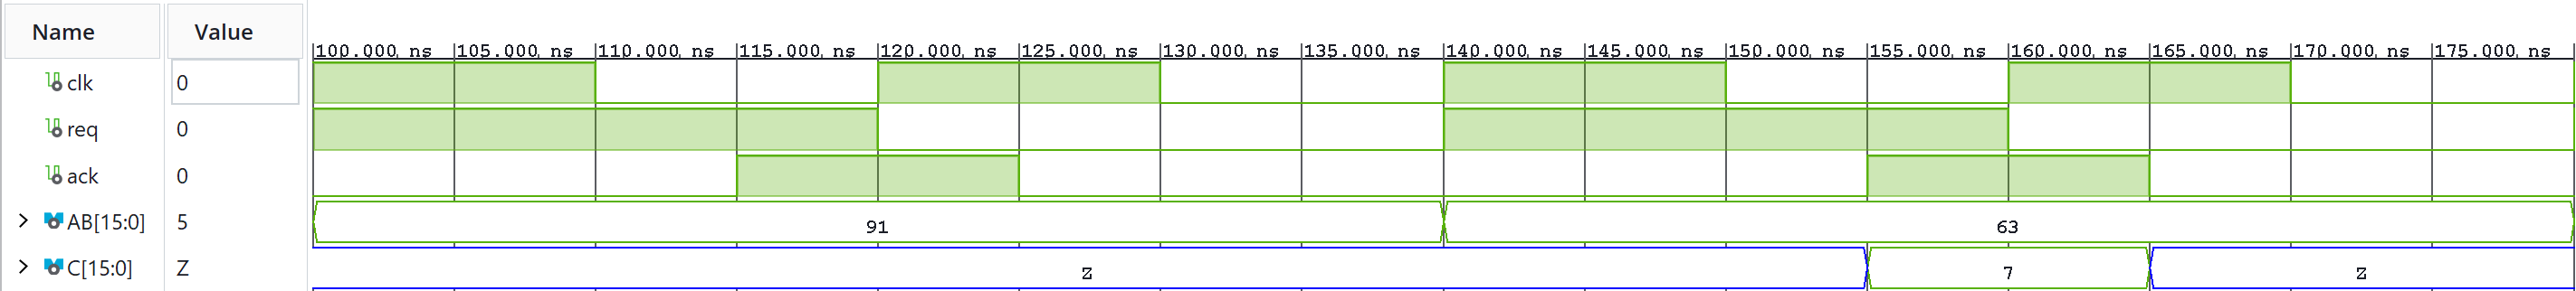
\includegraphics[width=\textwidth]{figures/task1_waveform.png}
  \caption{Passing Task 1 simulation waveform. The two request--acknowledge handshakes are visible for each operand pair, followed by the valid GCD result on \texttt{C}.}
  \label{fig:task1-waveform}
\end{figure}

\subsection{Handshake protocol}

The module interface follows a four-phase fully interlocked request--acknowledge protocol. The requester first raises \texttt{req} while placing a valid operand on \texttt{AB}. The module captures the operand and raises \texttt{ack} when it has accepted it. The requester then lowers \texttt{req}, and the module lowers \texttt{ack}, completing that handshake. The same sequence is performed a second time for operand $B$; after accepting it, the module computes the GCD and keeps the result valid on \texttt{C} while \texttt{ack} is high. The requester lowers \texttt{req}, after which the module lowers \texttt{ack} and removes the result from the output. The initial handshake transfers $A$, while the second handshake transfers $B$ and returns the result.